The eigenspaces of conservation laws systems defined above will be now investigated. As we shall see, the characteristic structure of those problems may lead to different type of waves propagating within a medium. Finally, existing analytical solutions of one-dimensional problems \cite{Wang} will be reviewed and that of a one-dimensional problem involving a hyperelastic \textit{Saint-Venant--Kirchhoff} material will be developed in order to illustrate the identified wave structures.
\subsection{Characteristic structure of solutions}
For the sake of simplicity studies of finite deformation and linearized geometrical frameworks will be condensed in this part by using a generic stress measure $\tens{S}$ and vectors written in the reference configuration. Furthermore, instead of studying multi-dimensional conservation laws systems, we will focus without loss of generality on conservative forms \eqref{eq:general_conservative} projected on an arbitrary direction $\vect{N}=\[\vect{e}_1,\vect{e}_2,\vect{e}_3\]$ \cite[p.425-426]{Leveque}. In this direction, the quasi-linear forms determined above are rewritten as:
\begin{equation}
  \label{eq:normal_quasi}
  \Qcb_t + \Jbsf \drond{\Qcb}{X_N} = \Scb
\end{equation}
where $X_N=\vect{X}\cdot\vect{N}$ and the \textit{Jacobian matrix} $\Jbsf = \Absf^\alpha N_\alpha$ of dimension $m$ arise. Hence, the characteristic analysis of system \eqref{eq:normal_quasi} is equivalent to that of linear combinations of matrices $\Absf^\alpha$. With the previous developments, the Jacobian matrix reads:
\begin{equation}
  \label{eq:jacobian_generic}
  \Jbsf=-\matrice{\tens{0}^2 & \frac{1}{\rho_0}\tens{I}\otimes \vect{N} \\  \tilde{\Hbb}\cdot\vect{N} & \tens{0}^4 }
\end{equation}
in which $\tilde{\Hbb}$ is either the hyperelastic or elastoplastic tangent modulus, or the elastic stifness tensor depending on the case considered. For general three-dimensional case, the characteristic structure of the problem is given by the $12$ eigenvalues $c_k$ and associated left eigenvectors $\Lcb^k$ of the Jacobian matrix:
\begin{equation}
  \label{eq:eigen_system}
  \vect{\Lc}^k\cdot \(\Jbsf - c_k \Ibsf\) = \vect{0}
\end{equation}
where $\Ibsf$ is the identity matrix and $\vect{\Lc}^k= \[ \vect{v}^K \: , \: \tens{S}^K \]$, with $\tens{S}$ standing for the suitable stress mesure. Thus, for non-null eigenvalues one gets:
\begin{subequations}
  \begin{alignat}{1}
    \label{eq:eigen_left_stress}
    & -\tens{S}^k:\(\tilde{\Hbb}\cdot  \vect{N}\) - c_k  \vect{v}^k =\vect{0} \\
    \label{eq:eigen_left_velo}
    & -\frac{1}{\rho_0}\vect{v}^k\otimes\vect{N} - c_k \tens{S}^k = \tens{0}
  \end{alignat}
\end{subequations}
Substitution of $\tens{S}$ obtained from \eqref{eq:eigen_left_velo} in \eqref{eq:eigen_left_stress} leads to:
\begin{equation}
  \label{eq:acoustic_eigen}
 (\vect{v}^k\otimes\vect{N}):\(\tilde{\Hbb}\cdot  \vect{N}\) - \rho_0\lambda^2_k \vect{v}^k = \tens{0}
\end{equation}
System \eqref{eq:acoustic_eigen} is the \textit{acoustic tensor} $A_{ij}=N_\alpha \tilde{H}_{i\alpha j \beta}  N_\beta$ left eigensystem which, due to the symmetry of $\tens{A}$ is equivalent to the right eigensystem:
\begin{equation}
  \label{eq:acoustic_eigen_system_lambda}
  \(  N_\alpha \tilde{H}_{i\alpha j \beta}  N_\beta - \rho_0 c_k^2 \delta_{ij} \) v_j^k =0
\end{equation}
or atlernatively with the eigenvalues $\omega_p$ and associated left eigenvectors of the acoustic tensor $\vect{l}^p\: \: (p=1,2,3)$:
\begin{equation}
  \label{eq:acoustic_eigen_system}
  \( \tens{A} - \omega_p \tens{I} \) \vect{l}^p = \vect{0}
\end{equation}
The condition for system \eqref{eq:normal_quasi} to be hyperbolic and have real eigenvalues and associated eigenvectors is thus ensured by the positive definiteness of the acoustic tensor, also known as the \textit{strong ellipticity} condition \cite{Foundation_of_elasticity}:
\begin{equation}
  \label{eq:strong_ellipticity}
  (\vect{m}\otimes \vect{N}): \tilde{\Hbb}: (\vect{m}\otimes \vect{N}) > 0 \quad \forall \vect{N},\vect{m} \in \Rbb^3 \: ; \: \vect{N},\vect{m} \ne \vect{0}
\end{equation}
If the condition holds, the acoustic tensor admits $3$ couples eigenvalues--eigenvectors $\{\omega_p,\vect{l}^p\}$ leading to $6$ couples $\{c_k,\Lcb^k\}$ for the Jacobian matrix, the $6$ other eigenvalues being null \cite{Kluth}. The couples $\{c_k,\Lcb^k\}$ are referred to as \textit{left characteristic fields}. The left eigenvectors associated to non-zero eigenvalues of the Jacobian matrix are obtained by using equation \eqref{eq:eigen_left_velo} so that the following $6$ eigenfields of quasi-linear form \eqref{eq:normal_quasi} can be defined:
\begin{equation}
  \label{eq:left_eigenfields}
    \left\lbrace \pm \sqrt{\frac{\omega_p}{\rho_0}} ; \quad \[\: \pm \rho_0\sqrt{\frac{\omega_p}{\rho_0}} \vect{l}^p , -\vect{l}^p\otimes \vect{N} \:\]  \right\rbrace ,\quad p=1,2,3
\end{equation}
At last, one has to find six independent left eigenvectors associated to the null eigenvalue of multiplicity $6$ by solving equation of \eqref{eq:eigen_left_stress} for the null eigenvalue:
\begin{equation}
  \label{eq:left_null_eigenvectors}
  \tens{S}^k:\(\tilde{\Hbb}\cdot  \vect{N}\) =\vect{0},\quad k=1,...,6
\end{equation}
Following the same procedure for right eigenvectors $\Rcb^k=\matrice{\vect{v}^k \\ \tens{S}^k}$, the Jacobian matrix right eigensystem reads:
\begin{subequations}
  \begin{alignat}{1}
    \label{eq:eigen_right_stress}
    & -\frac{1}{\rho_0}\tens{S}^k\cdot  \vect{N} - c_k  \vect{v}^k =\vect{0} \\
    \label{eq:eigen_right_velo}
    & -\tilde{\Hbb}:\(\vect{v}^k\otimes\vect{N}\) - c_k \tens{S}^k = \tens{0}
  \end{alignat}
\end{subequations}
which leads to the \textit{right eigen fields} associated to the non-null eigenvalues:
\begin{equation}
  \label{eq:right_eigenfields}
  \left\lbrace \pm \sqrt{\frac{\omega_p}{\rho_0}} ; \quad \[\: \pm \sqrt{\frac{\omega_p}{\rho_0}} \vect{l}^p , -\tilde{\Hbb}:\( \vect{l}^p\otimes \vect{N}\) \:\]  \right\rbrace ,\quad p=1,2,3
\end{equation}
In equation \eqref{eq:right_eigenfields}, $\{\omega_p,\vect{l}^p\}$ still denotes the eigenfields of the acoustic tensor. Moreover, the $6$ independent right eigenvectors associated to the zero eigenvalue required to complete the set of right characteristic fields must satisfy:
\begin{equation}
  \label{eq:right_null_eigenvectors}
  \tens{S}^k \cdot  \vect{N} =\vect{0},\quad k=1,...,6
\end{equation}

Note that since the right-hand side of equation \eqref{eq:normal_quasi} is not involved in the characteristic analysis, linear elasticity and elaso-viscoplasticity leads to the same characteristic structure. Furthermore, the specialization of characteristic equations along characteristic curves \eqref{eq:PDEs_ODEs} to system \eqref{eq:normal_quasi} leads to:
\begin{equation}
  \label{eq:characteristic_equations_homogeneous}
  \Lcb^k \cdot d\Qcb = \vect{0},\quad k=1,...,6
\end{equation}
meaning that the solution is constant along each ray $\xi = x/t$ through the origin. Solutions $\Qcb(\xi)$ are then called \textit{similarity solutions} and allow to rewrite the quasi-linear form as:
\begin{equation}
  \label{eq:quasi-linear_similarity}
  -\frac{x}{t^2}\Qcb'(\xi) + \Jbsf \frac{1}{t}\Qcb'(\xi) = \vect{0} \quad \Rightarrow \quad \(\Jbsf- \xi \:\Ibsf \) \Qcb'(\xi) = \vect{0}
\end{equation}
By looking at characteristic curves $\xi=c_k$, system \eqref{eq:quasi-linear_similarity} implies that $\Qcb'$ is equivalent to the right eigenvector $\Rcb^k$ and integration of $\Qcb'$ yields an \textit{integral curve} that is tangent at every point of the \textit{phase plane} $\(\Qcb_1,...,\Qcb_{m}\)$ to this eigenvector.

$\newline$
The notions highlighted so far will be illustrated in the two following sections. The method of characteristics will lead to:
\begin{itemize}
\item[(i)] the well-known solution to the \textit{Riemann problem} on a elastic bar
\item[(ii)] the development of the solution the Riemann problem of a hyperelastic Saint-Venant-Kirchhoff medium undergoing a one-dimensional strain state
\end{itemize}
Furthermore, the \textit{Rankine-Hugoniot condition} for discontinuous waves, and the concept of \textit{shock} and \textit{simple} waves will be introduced.

\subsection{Linear problems}
A Riemann problem is a Cauchy problem composed of a hyperbolic system and piecewise constant initial data on both sides of an interface. In the arbitrary direction $\vect{N}=\[\vect{e}_1,\vect{e}_2,\vect{e}_3\]$, the Riemann problem reads:
\begin{equation}
  \label{eq:Riemann_problem}
  \begin{aligned}
  &\Qcb_t + \drond{\Fcb\cdot \vect{N}}{X_N} = \Scb, \\
  &\left\lbrace 
    \begin{aligned}
      & \Qcb(X_N,t=0) = \Qcb_L \quad \text{if } X_N< 0\\
      & \Qcb(X_N,t=0) = \Qcb_R \quad \text{if } X_N> 0
    \end{aligned}
    \right.
  \end{aligned}
\end{equation}

We consider a one-dimensional elastic medium of density $\rho$ undergoing one-dimensional stress and strain states within the infinitesimal framework: $\tens{\eps}=\eps\: \vect{e}_1\otimes \vect{e}_1$ ; $\tens{\sigma}=\sigma \:\vect{e}_1\otimes \vect{e}_1$, so that the bar hypothesis holds with $\vect{v}=v \vect{e}_1$. The Riemann problem consists then of problem \eqref{eq:Riemann_problem} for $\vect{N}=\vect{n}=\vect{e}_1$ and $X_N=x$.

Neglecting body forces without loss of generality and introducing \textit{Yound's modulus E} such that $\sigma = E\eps$, conserved quantities and flux vector are:
\begin{equation*}
  \Qcb = \matrice{v \\ \sigma} \quad ; \quad \Fcb = \matrice{-\frac{1}{\rho}\sigma \\ -Ev}
\end{equation*}
The eigenvalues and left eigenvectors of the corresponding Jacobian matrix are:
\begin{equation*}
  c_{1,2} = \pm \sqrt{\frac{E}{\rho}}=\pm c \quad ; \quad \Lcb^p=\[\rho c_p \:,\: -1\] \quad ; \quad \Rcb^p=\matrice{1\\- \rho c_p } 
\end{equation*}

\subsubsection*{The method of characteristics}
The system of ODE along the characteristic curves, given by characteristic equations \eqref{eq:PDEs_ODEs}, is:
\begin{equation}
  \label{eq:elast_charac_equation}
  \Lcb^p \cdot d\Qcb = 0 \quad \Rightarrow
  \left\lbrace
    \begin{aligned}
      & \rho c\: dv - d\sigma = 0\\
      -& \rho c\: dv - d\sigma = 0
    \end{aligned} \right.
\end{equation}
Consider now a point $P$ of the ($x,t$) plane at which we are looking for the solution. Applying the method of characteristic, we trace the two characteristic straight lines starting from the $x$-axis (along which $\Qcb$ is given) and passing through $P$ (dashed lines in figure \ref{fig:elasticity_example}).  
\begin{figure}[h]
  \centering
  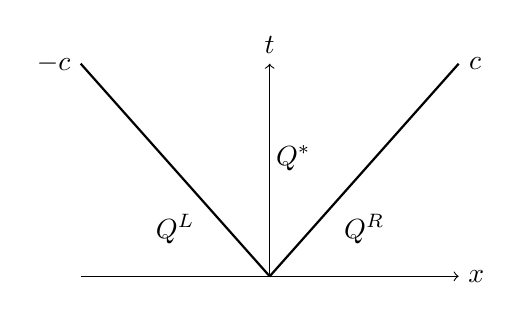
\begin{tikzpicture}[scale=0.6]
  \draw[->] (-4,0) -- (4.,0) node[right] {$x$};
  \draw[->] (0,0) -- (0,4.5) node[above] {$t$};
  \draw[thick] (0,0) -- (4.,4.5) node [right] {$c$};
  \draw[thick] (0,0) -- (-4.,4.5) node [left] {$-c$};
  \node at (2.,1.) {$\vect{Q}^R$};
  \node at (-2.,1.) {$\vect{Q}^L$};
  \node at (0.5,2.5) {$\vect{Q}^*$};
\end{tikzpicture}



%%% Local Variables:
%%% mode: latex
%%% TeX-master: "../../mainManuscript"
%%% End:

  \caption{Solution to Riemann problem \eqref{eq:Riemann_problem} for an elastic bar.}
  \label{fig:elasticity_example}
\end{figure}
Integration of characteristic equations \eqref{eq:elast_charac_equation} respectively along $AP$ and $BP$ yields:
\begin{equation}
  \label{eq:elastic_integral_curves}
  \left\lbrace
    \begin{aligned}
      & \rho c \(v_P - v_A \) - \(\sigma_P - \sigma_A \) = 0\\
      -& \rho c \(v_P - v_B \) - \(\sigma_P - \sigma_B \) = 0
    \end{aligned}
    \right.
\end{equation}
which solution is:
\begin{equation}
  \label{eq:elastic_solution_P}
  v_P = \frac{\sigma_B - \sigma_A}{2\rho c} + \frac{v_A+v_B}{2} \quad ; \quad \sigma_P = \rho c\frac{v_B - v_A}{2} + \frac{\sigma_A+\sigma_B}{2}
\end{equation}
On the other hand, the same procedure for point $P'$ leads to the solution:
\begin{equation}
  \label{eq:elastic_solution_Q}
  v_{P'} = \frac{\sigma_B - \sigma_{A'}}{2\rho c} + \frac{v_{A'}+v_B}{2} \quad ; \quad \sigma_{P'} = \rho c\frac{v_B - v_{A'}}{2} + \frac{\sigma_{A'}+\sigma_B}{2}
\end{equation}
With initial data given for the Riemann problem, it appears that $\Qcb_{A'}=\Qcb_{B}$ and hence, $\Qcb_{P'}=\Qcb_{R} \ne \Qcb_{P}$. Let's assume now that points $P$ and $P'$ are still on each side of the right characteristic straight line emanating from the origin but infinitely close to it. It is obvious that the previous results hold and that the a jump discontinuity propagates in the bar with speed $c$. Hence, we are left with the following condition across a discontinuous wave \cite{Toro} that generalizes to all linear Riemann problems:
\begin{definition}
Given a system of hyperbolic conservation laws $\Qcb_t + \Fcb(\Qcb)_x=\vect{0}$ and a discontinuous wave solution of speed $s_i$ associated to the $i$th characteristic field, the \textbf{Rankine-Hugoniot condition} reads:
\begin{equation}
  \label{eq:rankine-hugoniot}
  \saut{ \Fcb} = s_i \saut{ \Qcb}
\end{equation}
where $\saut{\bullet}$ denotes the jump operator across the discontinuity.  
\end{definition}

\subsubsection*{Characteristic variables -- Waves solution}
By introducing a set of \textbf{characteristic variables} $\Hcb=\Rbsf^{-1}\Qcb$, where $\Rsf_{ij}=\Rc^j_i$ is the matrix of right eigenvectors, the quasi-linear form of system \eqref{eq:Riemann_problem} can be rewritten as a system of decoupled scalar linear advection equations.
% \begin{equation}
%   \label{eq:scalar_1st_order_pdes}
%   \Hcb_t + \Cbsf\Hcb_x = \vect{0}
% \end{equation}
The Riemann problem can then be formulated in terms of characteristic variables:
\begin{equation*}
  \begin{aligned}
    &\Hcb_t + \Cbsf\Hcb_x = \vect{0} \\
    &\left\lbrace 
      \begin{aligned}
        & \Hcb(x,t=0) = \Hcb_L \quad \text{if } x< 0\\
        & \Hcb(x,t=0) = \Hcb_R \quad \text{if } x> 0
      \end{aligned}
    \right.
  \end{aligned}
\end{equation*}
with $\Csf_{ij}=c_i\delta_{ij}$ so that $\Jsf_{ij} \Rc^j_k = \Rc^k_i\Csf_{kj}$. 

The solution to such a problem is straightforward since it can be seen as the superposition of problems involving only one wave.
\begin{equation*}
  \Hc_i(x,t)=\left\lbrace
    \begin{aligned}
      & {\Hc_i}_L \quad \text{if } \:x <c_i t\\
      & {\Hc_i}_R \quad \text{if } \:x>c_i t
    \end{aligned}
  \right. %= \Hc_i(x-c_it,0)
\end{equation*}
Hence, by inverting the relation:
\begin{equation*}
  \Qcb = \Rcb^j \Hc_j(x,t) = \Rcb^j\Hc_j(x-c_jt,0)
\end{equation*}
where the $\Hc_j(x-c_jt,0)$ appear as coefficients of an eigenvector expansion.

\todo{Have to introduce the eigenvector expension so the shock wave solution can be developed}
\subsection{Non-linear problems}
We now consider a hyperelastic medium made of a Saint-Venant-Kirchhoff material, infinite in directions $\vect{e}_2$ and $\vect{e}_3$, and semi-infinite in direction $\vect{e}_1$ (\textit{i.e. $x_1 \in [0,+\infty[$}). This medium undergoes a load at $X_1=X=0$ in direction $\vect{e}_1$ so that the deformation gradient and the PK1 tensor are respectively:
\begin{align*}
  &\tens{F}=F\vect{e}_1\otimes\vect{e}_1 + \vect{e}_2\otimes\vect{e}_2 + \vect{e}_3\otimes\vect{e}_3 \\
  & \tens{\Pi}=\Pi_{11}\vect{e}_1\otimes\vect{e}_1 + \Pi_{22}\(\vect{e}_2\otimes\vect{e}_2 + \vect{e}_3\otimes\vect{e}_3 \)
\end{align*}
which corresponds to a plane wave solution. Once again, the Riemann problem considered is \eqref{eq:Riemann_problem} in which $\vect{N}=\vect{e}_1$ and:
\begin{equation*}
 \Qcb = \matrice{v \\ F} \quad ; \quad \Fcb = \matrice{-\frac{1}{\rho_0}\Pi \\ -v}
\end{equation*}
with neglected body forces and $\Pi=\Pi_{11}$. With tangent modulus and acoustic tensor of Saint-Venant-Kirchhoff model \eqref{eq:SVK_tangent},\eqref{eq:SVK_acoustic} depending on the deformation gradient, the integration of characteristic equations is simpler with the quasi-linear form: $\Qcb_t + \drond{\Fcb}{\Qcb}\drond{\Qcb}{X}=\vect{0}$ where:
\begin{equation}
  \label{eq:quasi_SVK}
  \Jbsf=\drond{\Fcb}{\Qcb}=-\matrice{0 & -\frac{H_{1111}}{\rho_0} \\ 1 & 0}
\end{equation}
The characteristic fields of this system are:
\begin{equation}
  \label{eq:SVK_charac_fields}
  c_{1,2}=\pm \sqrt{\frac{\lambda+2\mu}{2\rho_0}\(3F^2-1\) } \quad ; \quad \Lcb^p=\[1\:,\:- c_p \] \quad ; \quad \Rcb^p=\matrice{- c_p \\1} 
\end{equation}
The non-linear flux function (\textit{i.e.} $\ddrond{\Pi_{11}}{F}{F}\neq 0$) yields characteristic fields depending on the strain state and, for the Saint-Venant--Kirchhoff model, possibly complex celerities leading to a loss of hyperbolicity of the problem for $F>\sqrt{\frac{1}{3}}$.
\begin{figure}[h]
  \centering
  \subfloat[Left-going shock \label{subfig:1S}]{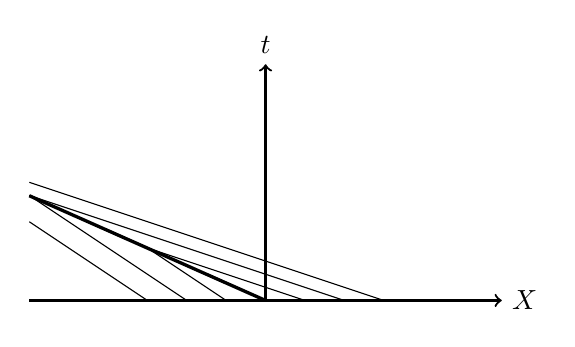
\begin{tikzpicture}
  \draw[->,thick] (-3,0) -- (3,0) node[right] {$X$};
  \draw[->,thick](0,0) -- (0,3) node[above] {$t$};
  \draw(-0.5,0) -- (-1.5,2/3) ;
  \draw(-1,0) -- (-3.,4./3) ;
  \draw(-1.5,0) -- (-3.,1.) ;
  \draw(0.5,0) -- (-1.5,2./3.) ;
  \draw(1.,0) -- (-3.,4./3) ;
  \draw(1.5,0) -- (-3.,3./2) ;
  \draw[very thick] (0,0) -- (-3,1.33);
\end{tikzpicture}}
  \subfloat[Right-going simple wave \label{subfig:2R}]{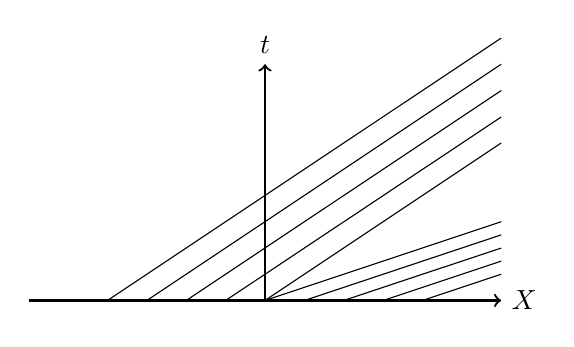
\begin{tikzpicture}
  \draw[->,thick] (-3,0) -- (3,0) node[right] {$X$};
  \draw[->,thick](0,0) -- (0,3) node[above] {$t$};
  \draw(0,0) -- (3,2) ;
  \draw(-0.5,0) -- (3,2.33) ;
  \draw(-1,0) -- (3,2.666) ;
  \draw(-1.5,0) -- (3,3) ;
  \draw(-2,0) -- (3,3.333) ;
  \draw(0,0) -- (3,1) ;
  \draw(0.5,0) -- (3,0.833) ;
  \draw(1,0) -- (3,0.666) ;
  \draw(1.5,0) -- (3,0.5) ;
  \draw(2,0) -- (3,0.333) ;
\end{tikzpicture}}
  \caption{Wave pattern generated by initial data of the Riemann problem such that $F_L<F_R$: 1--shock ; 2--rarefaction.}
  \label{fig:1S2R}
\end{figure}

Initial conditions have an influence on the characteristic structure of the solution due to the dependence of characteristic speeds on the deformation gradient. Indeed, if initial data are given so that $F_L < F_R$, the resulting characteristic speeds satisfy $c_1(F_L)<c_1(F_R) \: ; \: c_2(F_L)<c_2(F_R)$. Hence, the 1-characteristic fields move away from each other in the right region of the ($x,t$) plane (figure \ref{fig:1S2R}\subref{subfig:2R}) while the 2-characteristic fields collide in the left region (figure \ref{fig:1S2R}\subref{subfig:1S}). Those two situations respectively correspond to simple and shock waves.

\subsubsection*{Shock waves}
By applying the method of characteristics between the $x$-axis and an intersection point of two characteristic straight lines allows to show that a shock wave carry a jump discontinuity of the conserved quantity vector and hence, satisfy the Rankine-Hugoniot condition \eqref{eq:rankine-hugoniot} where the shock speed $s_i$ is to be defined. Assuming that a shock wave separates a region of the ($x,t$) plane in which $\Qcb=\bar{\Qcb}$ is known (initial conditions) from another where $\Qcb=\tilde{\Qcb}$ is to be defined. According to Rankine-Hugoniot conditions, those states obey:
\begin{align}
  \label{eq:RH_velocity}
  & -\frac{1}{\rho_0}\(\tilde{\Pi} - \bar{\Pi} \) = s \( \tilde{v} - \bar{v} \)\\
  \label{eq:RH_F}
  & - \( \tilde{v}-\bar{v}\)=s\( \tilde{F} - \bar{F}\)
\end{align}
Substitution of $s$ from equation \eqref{eq:RH_F} and introduction in equation \eqref{eq:RH_velocity} where $\Pi=\frac{\lambda+2\mu}{2}\(F^3-F\)$ yield:
\begin{align}
  \label{eq:shock_speed}
  & s=-\frac{\tilde{v}-\bar{v}}{\tilde{F} - \bar{F}}\\
  \label{eq:v_jump}
  & \tilde{v}-\bar{v}= \pm \sqrt{\frac{\lambda+2\mu}{2\rho_0}(\tilde{F}-\bar{F})\[ \tilde{F}^3-\tilde{F} - (\bar{F}^3-\bar{F})\]}
\end{align}
Equation \eqref{eq:v_jump} yields two families of curves in the phase plane associated to either $\Rcb^1$ or $\Rcb^2$


In addition to the Rankine-Hugoniot condition, the \textit{Lax entropy condition} stating that characteristic curves collide in a shock wave must be satisfied:
\begin{equation}
  \label{eq:Lax_entropy}
  \lambda(\bar{F})<s<\lambda(\tilde{F})
\end{equation}
For a Saint-Venant--Kirchhoff material, the Lax condition leads to $\bar{F} > \tilde{F}$ ensuring thus that the square root in equation \eqref{eq:v_jump} is real.

\subsubsection*{Simple waves}


\begin{figure}[h]
  \centering
  \subfloat[Left-going simple wave \label{subfig:1R}]{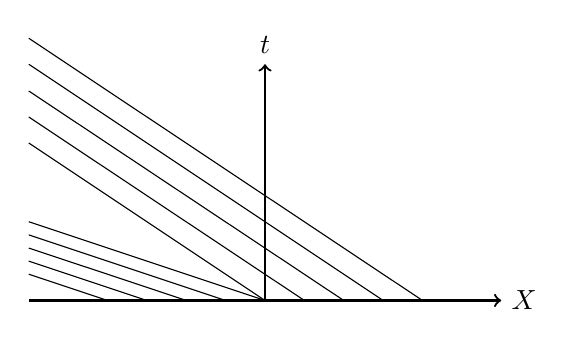
\begin{tikzpicture}
  \draw[->,thick] (-3,0) -- (3,0) node[right] {$X$};
  \draw[->,thick](0,0) -- (0,3) node[above] {$t$};
  \draw(0,0) -- (-3,1) ;
  \draw(-0.5,0) -- (-3,0.833) ;
  \draw(-1,0) -- (-3,0.666) ;
  \draw(-1.5,0) -- (-3,0.5) ;
  \draw(-2,0) -- (-3,0.333) ;
  \draw(0,0) -- (-3,2) ;
  \draw(0.5,0) -- (-3,2.33) ;
  \draw(1.,0) -- (-3,2.66) ;
  \draw(1.5,0) -- (-3,3) ;
  \draw(2.0,0) -- (-3,3.33) ;
\end{tikzpicture}}
  \subfloat[Right-going shock \label{subfig:2S}]{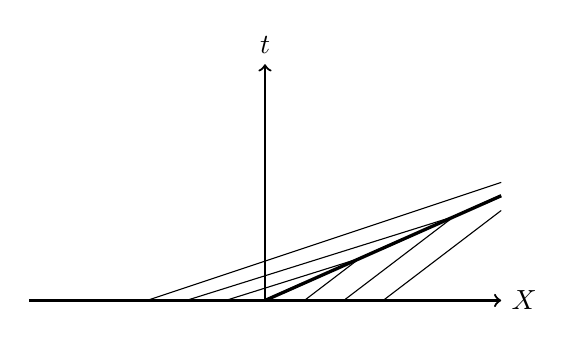
\begin{tikzpicture}
  \draw[->,thick] (-3,0) -- (3,0) node[right] {$X$};
  \draw[->,thick](0,0) -- (0,3) node[above] {$t$};
  \draw(-0.5,0) -- (1.20,0.533333) ;
  \draw(-1,0) -- (2.40,1.066) ;
  \draw(-1.5,0) -- (3,1.5) ;
  %\draw(-2,0) -- (3,1.666) ;
  %%%%%%%%% 
  \draw(0.5,0) -- (1.20,0.533333) ;
  \draw(1.,0) -- (2.40,1.066) ;
  \draw(1.5,0) -- (3,1.14285) ;
  %\draw(2.0,0) -- (3,0.7619) ;
  \draw[very thick] (0,0) -- (3,1.33);
\end{tikzpicture}}
  \caption{Wave pattern generated by initial data of the Riemann problem such that $F_L>F_R$: 1--rarefaction ; 2--shock.}
  \label{fig:1R2S}
\end{figure}
the negative eigenvalue will be lower for $X<0$ than for $X>0$, leading to colliding characteristic fields in the left region (figure \ref{fig:1S2R}\subref{subfig:1S}), generating thus a \textit{shock wave}. Applying the method of characteristics between the $x$-axis and an intersection point of two characteristic straight lines allows to show that a shock wave carry a jump discontinuity of the conserved quantity vector and hence, satisfy the Rankine-Hugoniot condition \eqref{eq:rankine-hugoniot} where the shock speed $s_i$ is to be defined.

On the other hand, those initial conditions lead to right-going characteristics moving away from each other. Such a characteristic structure corresponds to a \textit{simple wave} (see figure \ref{fig:1S2R}\subref{subfig:2R}), which in case of a vanishing right-hand side of the hyperbolic system becomes a \textit{rarefaction wave} (\textit{i.e. a simple wave propagating a self-similar solution $\Qcb(\xi)$}). The characteristic structure of the solution corresponding to initial data such that $F_L > F_R$, depicted in figure \ref{fig:1R2S}, consists in a left-going rarefaction and a right-going shock waves. 

$\newline$
Note that the above discussion holds for concave flux functions which is not the case for the neo-Hookean model for instance. Indeed, such a model yields a monotonically decreasing positive characteristic speeds with the gradient of deformation (see figure \ref{fig:SVK-NH}\subref{subfig:SVK_NH_speeds}). Hence, initial data considered previously will lead to opposite situations (\textit{i.e. $F_L<F_R \rightarrow $ 1--rarefaction ; 2--shock, and $F_L>F_R \rightarrow $ 1--shock ; 2--rarefaction}). Moreover, the polyconvexity of the neo-Hookean stored energy function ensures the hyperbolicity of the system so that the problem does not suffer any limitation on the deformation gradient.
\begin{figure}[h]
  \centering
  \subfloat[Stress $\Pi_{11}$ \label{subfig:SVK_NH_Pi}]{\definecolor{Red}{RGB}{217,33,32}
\definecolor{Blue}{RGB}{63,96,174}
\definecolor{Duck}{RGB}{83,158,182}
\definecolor{Green}{RGB}{109,179,136}
\definecolor{Yellow}{RGB}{202,184,67}
\definecolor{Orange}{RGB}{231,133,50}
\definecolor{Red}{RGB}{217,33,32}
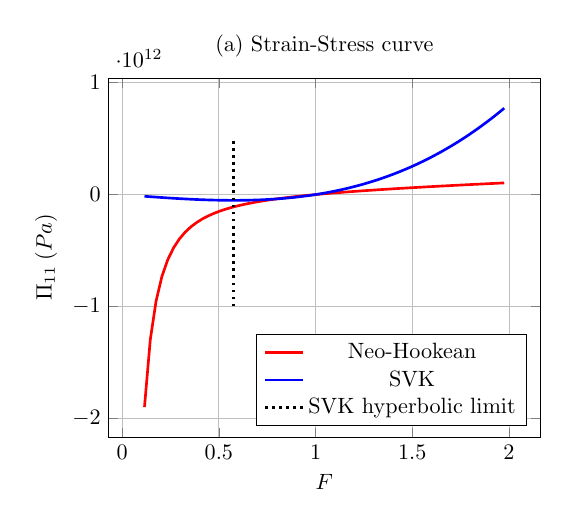
\begin{tikzpicture}[scale=0.8]
\begin{axis}[xlabel=$F$,ylabel=$\Pi_{11} \: (Pa)$,ymajorgrids=true,xmajorgrids=true,legend pos=south east,title={(a) Strain-Stress curve}]
\addplot[Red,very thick] coordinates {(0.11547005383792518,-1898966453319.162) (0.14547005383792516,-1296837707486.0405) (0.17547005383792513,-951312235719.5623) (0.20547005383792513,-732355105152.6451) (0.23547005383792513,-583575852118.2125) (0.2654700538379251,-477087968993.8754) (0.2954700538379251,-397729449724.4541) (0.3254700538379251,-336642141070.28204) (0.35547005383792507,-288349957545.72546) (0.38547005383792504,-249309520683.61847) (0.415470053837925,-217140040714.9308) (0.44547005383792504,-190190468824.5224) (0.475470053837925,-167284549773.97247) (0.505470053837925,-147564580724.34894) (0.535470053837925,-130392343185.27245) (0.5654700538379249,-115284401045.16144) (0.595470053837925,-101868733030.67676) (0.625470053837925,-89854990617.66492) (0.6554700538379249,-79013679521.07468) (0.6854700538379249,-69161318053.14328) (0.7154700538379248,-60149680216.69014) (0.7454700538379249,-51857881714.88495) (0.7754700538379249,-44186477584.150566) (0.8054700538379248,-37053004869.531456) (0.8354700538379248,-30388577783.986546) (0.8654700538379249,-24135259235.847366) (0.8954700538379248,-18244011798.887867) (0.9254700538379248,-12673085866.843775) (0.9554700538379248,-7386740998.494719) (0.9854700538379247,-2354223588.251995) (1.0154700538379247,2451056537.9352818) (1.0454700538379247,7052193879.264957) (1.0754700538379247,11469332294.041113) (1.1054700538379247,15720112571.176903) (1.1354700538379248,19820042073.450085) (1.1654700538379246,23782801671.8228) (1.1954700538379246,27620501912.14364) (1.2254700538379246,31343897846.142628) (1.2554700538379246,34962570023.63762) (1.2854700538379247,38485077640.53793) (1.3154700538379245,41919088663.206696) (1.3454700538379245,45271490826.59238) (1.3754700538379245,48548486673.378265) (1.4054700538379246,51755675220.64049) (1.4354700538379246,54898122376.10795) (1.4654700538379246,57980421852.87309) (1.4954700538379244,61006748029.95563) (1.5254700538379244,63980901961.52675) (1.5554700538379245,66906351538.24785) (1.5854700538379245,69786266641.0072) (1.6154700538379245,72623549993.23035) (1.6454700538379243,75420864307.28705) (1.6754700538379244,78180656228.87244) (1.7054700538379244,80905177507.05946) (1.7354700538379244,83596503754.174) (1.7654700538379244,86256551106.45828) (1.7954700538379245,88887091051.8295) (1.8254700538379243,91489763653.42323) (1.8554700538379243,94066089365.83081) (1.8854700538379243,96617479614.0105) (1.9154700538379243,99145246281.97147) (1.9454700538379244,101650610238.83322) (1.9754700538379242,104134709013.2085) };
\addplot[Blue,very thick] coordinates {(0.11547005383792518,-15336791766.165447) (0.14547005383792516,-19168111304.289738) (0.17547005383792513,-22893685303.277996) (0.20547005383792513,-26491706070.822536) (0.23547005383792513,-29940365914.61566) (0.2654700538379251,-33217857142.349674) (0.2954700538379251,-36302372061.71689) (0.3254700538379251,-39172102980.40962) (0.35547005383792507,-41805242206.12016) (0.38547005383792504,-44179982046.540825) (0.415470053837925,-46274514809.36392) (0.44547005383792504,-48067032802.28176) (0.475470053837925,-49535728332.98665) (0.505470053837925,-50658793709.17089) (0.535470053837925,-51414421238.526794) (0.5654700538379249,-51780803228.74666) (0.595470053837925,-51736131987.522804) (0.625470053837925,-51258599822.54755) (0.6554700538379249,-50326399041.513176) (0.6854700538379249,-48917721952.112) (0.7154700538379248,-47010760862.036354) (0.7454700538379249,-44583708078.97849) (0.7754700538379249,-41614755910.630775) (0.8054700538379248,-38082096664.68549) (0.8354700538379248,-33963922648.83495) (0.8654700538379249,-29238426170.77144) (0.8954700538379248,-23883799538.187305) (0.9254700538379248,-17878235058.774815) (0.9554700538379248,-11199925040.226295) (0.9854700538379247,-3827061790.2340784) (1.0154700538379247,4262162383.5095387) (1.0454700538379247,13089555173.312326) (1.0754700538379247,22676924271.481888) (1.1054700538379247,33046077370.32594) (1.1354700538379248,44218822162.15218) (1.1654700538379246,56216966339.268196) (1.1954700538379246,69062317593.98189) (1.2254700538379246,82776683618.60081) (1.2554700538379246,97381872105.43274) (1.2854700538379247,112899690746.78526) (1.3154700538379245,129351947234.96603) (1.3454700538379245,146760449262.28293) (1.3754700538379245,165147004521.04358) (1.4054700538379246,184533420703.55563) (1.4354700538379246,204941505502.12674) (1.4654700538379246,226393066609.06476) (1.4954700538379244,248909911716.677) (1.5254700538379244,272513848517.2716) (1.5554700538379245,297226684703.1562) (1.5854700538379245,323070227966.6382) (1.6154700538379245,350066286000.0256) (1.6454700538379243,378236666495.6256) (1.6754700538379244,407603177145.7466) (1.7054700538379244,438187625642.6959) (1.7354700538379244,470011819678.7812) (1.7654700538379244,503097566946.3102) (1.7954700538379245,537466675137.5906) (1.8254700538379243,573140951944.9299) (1.8554700538379243,610142205060.6364) (1.8854700538379243,648492242177.0171) (1.9154700538379243,688212870986.3801) (1.9454700538379244,729325899181.0331) (1.9754700538379242,771853134453.2832) };
\addplot[dotted,very thick] coordinates {(sqrt(1./3.),-1.e12) (sqrt(1./3.),0.5e12)};
\legend{Neo-Hookean,SVK,SVK hyperbolic limit}
\end{axis}
\end{tikzpicture}
}
  \subfloat[Characteristic speeds\label{subfig:SVK_NH_speeds}]{\definecolor{Red}{RGB}{217,33,32}
\definecolor{Blue}{RGB}{63,96,174}
\definecolor{Duck}{RGB}{83,158,182}
\definecolor{Green}{RGB}{109,179,136}
\definecolor{Yellow}{RGB}{202,184,67}
\definecolor{Orange}{RGB}{231,133,50}
\definecolor{Red}{RGB}{217,33,32}
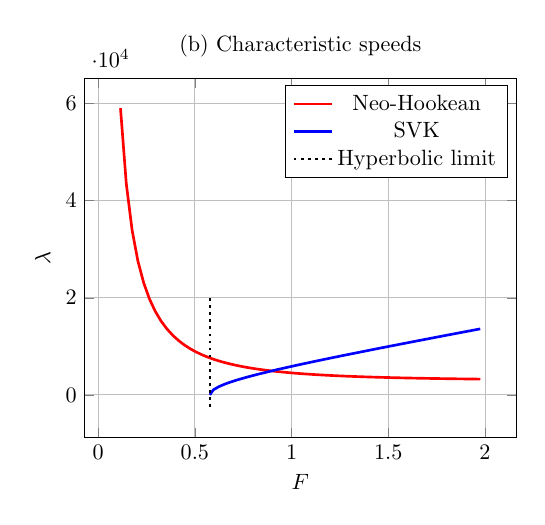
\begin{tikzpicture}[scale=0.8]
\begin{axis}[xlabel=$F$,ylabel=$\abs{\lambda}$,ymajorgrids=true,xmajorgrids=true,title={(b) Characteristic speeds}]
\addplot[Red,very thick] coordinates {(0.11547005383792518,59012.035730808406) (0.14547005383792516,43444.15680640866) (0.17547005383792513,33909.66271892359) (0.20547005383792513,27551.616086072518) (0.23547005383792513,23052.45426344622) (0.2654700538379251,19726.297080765253) (0.2954700538379251,17183.410876622853) (0.3254700538379251,15187.108927674422) (0.35547005383792507,13585.92851121213) (0.38547005383792504,12278.756336822797) (0.415470053837925,11195.691489974464) (0.44547005383792504,10286.970773511453) (0.475470053837925,9516.269220270638) (0.505470053837925,8856.492138358943) (0.535470053837925,8287.045413546242) (0.5654700538379249,7792.014425579814) (0.595470053837925,7358.918900548452) (0.625470053837925,6977.8428382999955) (0.6554700538379249,6640.81463208358) (0.6854700538379249,6341.3576871839605) (0.7154700538379248,6074.159484360366) (0.7454700538379249,5834.824367261866) (0.7754700538379249,5619.6864514897625) (0.8054700538379248,5425.666332338412) (0.8354700538379248,5250.16012367266) (0.8654700538379249,5090.952654625974) (0.8954700538379248,4946.148920983796) (0.9254700538379248,4814.119475233549) (0.9554700538379248,4693.456563660641) (0.9854700538379247,4582.938625301644) (1.0154700538379247,4481.501352586511) (1.0454700538379247,4388.21394243672) (1.0754700538379247,4302.259484218307) (1.1054700538379247,4222.918668359039) (1.1354700538379248,4149.556178447647) (1.1654700538379246,4081.609265724866) (1.1954700538379246,4018.57810915085) (1.2254700538379246,3960.0176447237714) (1.2554700538379246,3905.530610294456) (1.2854700538379247,3854.761601089376) (1.3154700538379245,3807.391969723345) (1.3454700538379245,3763.135435049281) (1.3754700538379245,3721.7342885593334) (1.4054700538379246,3682.9561065868374) (1.4354700538379246,3646.590892305437) (1.4654700538379246,3612.448584281259) (1.4954700538379244,3580.3568787248346) (1.5254700538379244,3550.1593210921387) (1.5554700538379245,3521.7136296737963) (1.5854700538379245,3494.8902195829423) (1.6154700538379245,3469.5709003379666) (1.6454700538379243,3445.6477242208375) (1.6754700538379244,3423.021965921998) (1.7054700538379244,3401.6032167766175) (1.7354700538379244,3381.308579249105) (1.7654700538379244,3362.061949309672) (1.7954700538379245,3343.793376030597) (1.8254700538379243,3326.438489161275) (1.8554700538379243,3309.9379866615427) (1.8854700538379243,3294.237175216221) (1.9154700538379243,3279.2855576483526) (1.9454700538379244,3265.0364619174256) (1.9754700538379242,3251.446707051308) };
\addplot[Blue,very thick] coordinates {(sqrt(1./3.),0.) (0.595470053837925,1048.9455179543422) (0.625470053837925,1731.1029259571128) (0.6554700538379249,2233.012146664284) (0.6854700538379249,2658.790029377158) (0.7154700538379248,3040.5889001561395) (0.7454700538379249,3393.286396027051) (0.7754700538379249,3725.1576526965905) (0.8054700538379248,4041.336632315833) (0.8354700538379248,4345.250197655363) (0.8654700538379249,4639.309436869055) (0.8954700538379248,4925.279696432755) (0.9254700538379248,5204.494537554574) (0.9554700538379248,5477.987035494905) (0.9854700538379247,5746.574266198714) (1.0154700538379247,6010.9138156437175) (1.0454700538379247,6271.542813975518) (1.0754700538379247,6528.905643538706) (1.1054700538379247,6783.374072186155) (1.1354700538379248,7035.262182069363) (1.1654700538379246,7284.837637447764) (1.1954700538379246,7532.330323596269) (1.2254700538379246,7777.939063134427) (1.2554700538379246,8021.836903239133) (1.2854700538379247,8264.175324905573) (1.3154700538379245,8505.087628335128) (1.3454700538379245,8744.691681060722) (1.3754700538379245,8983.092167747032) (1.4054700538379246,9220.382446402957) (1.4354700538379246,9456.646090866763) (1.4654700538379246,9691.958181097758) (1.4954700538379244,9926.386389147965) (1.5254700538379244,10159.991898394823) (1.5554700538379245,10392.830185782268) (1.5854700538379245,10624.951690800193) (1.6154700538379245,10856.402390269113) (1.6454700538379243,11087.224294354115) (1.6754700538379244,11317.455876364773) (1.7054700538379244,11547.132446624275) (1.7354700538379244,11776.286478876727) (1.7654700538379244,12004.947896244235) (1.7954700538379245,12233.144322567889) (1.8254700538379243,12460.901304010209) (1.8554700538379243,12688.242505014787) (1.8854700538379243,12915.189882077482) (1.9154700538379243,13141.763838254037) (1.9454700538379244,13367.983360890252) (1.9754700538379242,13593.866144695845) };
\addplot[dotted,very thick] coordinates {(sqrt(1./3.),-0.25e4) (sqrt(1./3.),2.e4)};
\legend{Neo-Hookean,SVK,Hyperbolic limit}
\end{axis}
\end{tikzpicture}
}
  \caption{Comparison of neo--Hookean and Saint-Venant--Kirchhoff hyperelastic models.}
  \label{fig:SVK-NH}
\end{figure}\todo{Give parameters values}
At last, figure \ref{fig:SVK-NH}\subref{subfig:SVK_NH_Pi} highlights the non-physical behaviour of Saint-Venant-Kirchhoff model for high compression loads that lead to a stress tensor tending to zero.

% Furthermore, the evolution of a characteristic speed along the associated integral curve is related to the following definitions:
% \begin{definition} A characteristic field is said to be \textbf{genuinely non-linear} if
%   \begin{equation}
%     \label{eq:linearly-degenerate}
%     \nablav_\Qc c_i \cdot \Rcb^i \neq \vect{0},\quad \forall \Qcb \in \Rbb^m
%   \end{equation}
% \end{definition}
% \begin{definition}
%   A characteristic field is said to be \textbf{linearly degenerate} if it satisfies
%   \begin{equation}
%     \label{eq:linearly-degenerate}
%     \nablav_\Qc c_i \cdot \Rcb^i = \vect{0},\quad \forall \Qcb \in \Rbb^m
%   \end{equation}
%   where $\nablav_\Ucb (\bullet)$ is the gradient in the phase plane. In particular, linear systems for which eigenvalues are constant, admit only linearly degenerate characteristic fields. An example of linearly degenerate field in a non-linear problem is that of contact discontinuities \cite[Chapter~13]{Leveque}.
% \end{definition}

% For the Saint-Venant-Kirchhoff material, equations \eqref{eq:SVK_charac_fields} lead to:
% \begin{equation*}
%   \nablav_\Qc c_p = \matrice{0\\ \frac{3(\lambda+2\mu)F}{2\rho_0c_p} } \quad \Rightarrow \nablav_\Qc c_p \cdot \Rcb^p = \frac{3(\lambda+2\mu)F}{2\rho_0c_p} 
% \end{equation*}
% with is not zero since $F>\sqrt{\frac{1}{3}}$.

While the solution through a shock wave can be determined with the Rankine-Hugoniot condition, the states connected to initial data through a rarefaction wave are given by integral curves. Indeed, since one seeks a similarity solution, the evolution of $\Qcb$ through a rarefaction wave obeys

\subsection{Integral curves}
\subsection{The Rankine-Hugoniot condition}


%%% Local Variables:
%%% mode: latex
%%% TeX-master: "../mainManuscript"
%%% End:
